基础设施是指Serverless底层的运行基础,
需要支持虚拟化/资源隔离/扩缩容等,
部分产品的架构选型如\cref{table:serverless-infras}所示。

\begin{table}[h!]
\centering
\begin{threeparttable}
    \begin{tabularx}{\textwidth}{|l|X|}
        \toprule
        \textbf{基础架构} & \textbf{产品} \\
        \midrule
        Kubernetes & 美团Nest\cite{meituan_serverless_nest, meituan_serverless_2}、
        字节ByteFaaS\cite{bytedance_faas}、Nimbella\cite{nimbella_k8s}、
        京东Serverless\cite{jd_serverless, jd_serverless_2} \\
        \hline
        Docker & 阿里函数计算\cite{aliyun_faas_arch_2}\tnote{1}、
        Oracle Functions\cite{overview_oracle_functions} \\
        \hline
        Knative & Google Cloud Run\cite{gcr_knative}、
        工商银行Serverless\cite{icbc_faas_arch}\tnote{1}、
        滴滴Serverless\cite{didi_serverless}  \\
        \hline
        Firecracker/microVM & AWS Lambda、AWS Fargate\cite{firecracker_home}、
        腾讯云函数\cite{tecent_faas_cold_start, tecent_serverless}\tnote{2} \\
        \hline
        Apache OpenWhisk & IBM Cloud Functions\cite{how_ibm_cloud_functions_works} \\
        \hline
        EasyFaaS & 百度函数计算CFC\cite{baidu_serverless_arch}、
        工商银行Serverless\cite{icbc_faas_arch} \\
        \bottomrule
    \end{tabularx}
\begin{tablenotes}
    \item[1] {\footnotesize 阿里函数计算第二代架构已经改为用神龙裸金属+安全容器实现\cite{aliyun_faas_arch_2}}
    \item[2] {\footnotesize 腾讯云使用自研的轻量级虚拟化技术,不确定是否与AWS microVM相同}
    \item[3] {\footnotesize 工商银行函数计算1.0使用Knative,2.0改用百度函数计算产品}
\end{tablenotes}
\end{threeparttable}
\caption{一些Serverless平台的基础设施}
\label{table:serverless-infras}
\end{table}

\subsubsection{基于Kubernetes}
Kubernetes已经是事实上的云原生标准,
因此使用Kubernetes作为底层运行时是一个最常规的选择,
且其本身自带了容器编排、服务治理等功能,生态较好。
Knative是谷歌开源的基于Kubernetes的Serverless运行环境。
因此有不少Serverless实现是使用Kubernetes作为运行时,
或者在此基础之上的Knative,
例如美团、字节以及谷歌等。

\subsubsection{基于裸金属+虚拟化技术}
使用裸金属服务器结合虚拟化技术(如安全容器或者MicroVM),
例如AWS Lambda和阿里函数计算等。
相对于Kubernetes而言,
这种方式弱化了集群管理的功能,
而将工作负载的管理交由Serverless平台处理,
更直接一些。
如AWS Lambda使用Firecraker/microVM实现工作负载,
如\cref{lambda_worker}所示。

\begin{figure}[ht!]
    \centering
    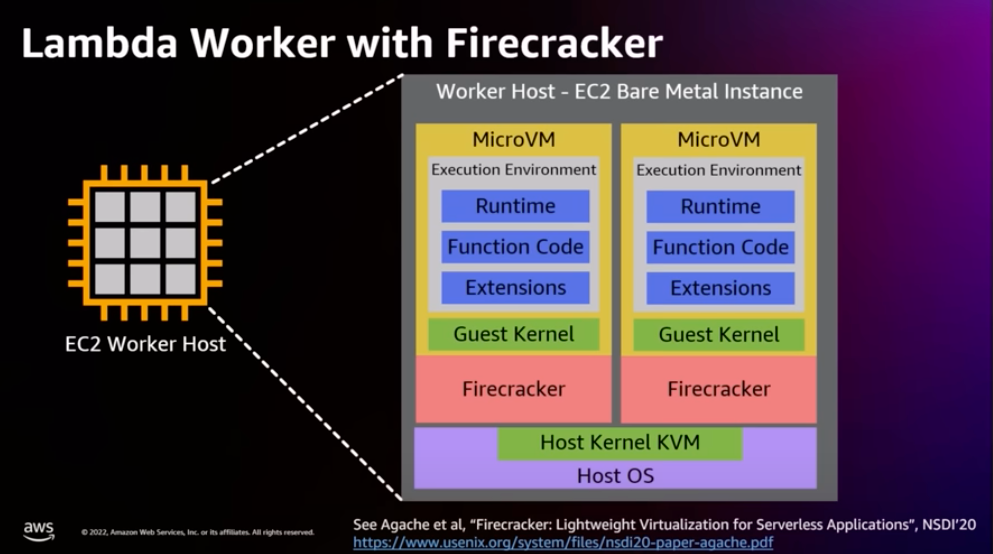
\includegraphics[width=0.7\linewidth]{images/lambda_worker.png}
    \caption{AWS Lambda的工作负载使用Firecracker虚拟化\cite{aws_lambda_2022}}
    \label{lambda_worker}
\end{figure}

除了AWS,阿里、腾讯等均采取了裸金属服务器+轻量级虚拟化技术的方式,
其中虚拟化技术又分为microVM或者安全容器两类。
除此之外,还有基于普通Docker实现的,
例如基于Docker的FaaS平台(如Fn Project)。

\subsubsection{混合使用Kubernetes及裸金属服务器}
除了上述的做法外,
还有一些框架也有支持多种运行时的,
例如Apache OpenWhisk、百度开源的EasyFaaS等,
采用框架封装支持多种运行时,可以混合使用Kubernetes以及Docker等。